
\documentclass[]{article}
\usepackage{mathrsfs}
\usepackage{amsmath}
\usepackage{graphicx}
\usepackage[top=1in,right=1in,left=1in,bottom=1in]{geometry}
\usepackage{setspace}
\usepackage{indentfirst}
\usepackage[margin=10pt,labelfont=bf,justification=raggedright,singlelinecheck=false]{caption}
\usepackage{color}
\usepackage{float}

\usepackage[pdftex]{hyperref}
\hypersetup{
       colorlinks=true,
       linkcolor=blue,
       citecolor=blue
}

\setlength{\abovecaptionskip}{6pt}   
\setlength{\belowcaptionskip}{6pt}   

% Begin
\begin{document}


%%%%%%%%%%%         PARAGRAPH SPACING       %%%%%%%%%%%%%%%%%%%%
% basically \doublespacing and \singlespacing. You can include them at any point in the document to change it for
% that point onward.
\doublespacing
\interfootnotelinepenalty=10000

% Set up a titlepage
\begin{titlepage}
\null\vspace{\stretch{1}}
\begin{center}
\textsc{\LARGE Environmental Sample Analysis by Means of Neutron Activation Analysis and Gamma-Ray Counting
}\\[1.5cm]

\textsc{\Large NE 170 Project Proposal}\\[0.5cm]
\textsc{\Large Eduardo Zagal, Peter Thomas, Shreyas Srinivasan, Zach Levine}\\[0.5cm] % Authors here
\textsc{\Large Advisers: Keenan Thomas and Professor Kai Vetter}\\[0.5cm]
\textsc{\Large April 28, 2016}\\[0.5cm] % Date that you turn it in
\end{center}
\vspace{\stretch{1}}
\end{titlepage}
\pagebreak


%%%%%%%%%%%%          TABLE OF CONTENTS          %%%%%%%%%%%%%%%%%%%%%%
\tableofcontents

%%%%%%%%%%%%%             PAGE BREAK            %%%%%%%%%%%%%%%%%
\pagebreak


%%%%%%%%%%%%          SECTION HEADINGS          %%%%%%%%%%%%%%%%%%%%%%
% To make section headings, use \section{Section Title}, adding a * makes a section title without numbering it.
% subsections are \subsection{Title} and \subsubsection{Title} and so on
\singlespacing

\section{Introduction}
Our team aims to determine the isotopic composition of kelp, fish, and other sea life along the west coast of the Americas, particularly in the San Francisco Bay and Long Beach, though we will be studying samples from Alaska all the way to Chile. In particular, we would like to see if there are any major differences in isotopes found in samples from different parts of the West Coast, and whether the isotopes found in the different samples will present a toxicity or radiological health hazard to the peoples living along the Pacific.

We will be using neutron activation analysis (NAA) to determine the isotopic composition of our samples. NAA involves irradiating test samples with a high neutron flux in order to activate the isotopes present in the sample. These isotopes then decay, emitting characteristic gamma rays that allow us to identify the isotopes that were originally in the sample. Based on the half-life of the isotope, its branching ratio at a particular gamma energy, and the counts registered on the detector, we can also determine the amount of the isotope in the test sample. NAA provides advantages that other techniques do not. NAA is relatively unobtrusive, and will not cause significant damage to the test sample. As neutrons can penetrate deeply into a material, NAA can be used on bulk samples. These samples do not need the careful preparation that is needed for other techniques to determine isotopic composition. Thus, NAA provides a fairly accurate and precise measurement of isotopic compositions without causing physical damage to the sample, and without the hassle of extended preparation time. With these advantages come some significant disadvantages that we will have to work around. One is that materials activated by neutrons remain radioactive for a long time after irradiation took place. Dependent on the isotopes in the sample, and the half-lives of those isotopes, this can make working with activated materials hazardous. This should not be an overwhelming concern for our team, as the samples that we will be working with are not expected to contain hazardous isotopes in the concentration needed to be harmful to us. Nevertheless, presence of toxic and radiologically active materials should be noted. The other concern is that there are only a select few facilities that have the capabilities needed to perform neutron activation on test samples. Fortunately, the McClellan Nuclear Research Center (MNRC), which is able to perform neutron activation, is relatively close, an advantage that will be crucial to the success of our project.

            



\section{Goals}

Our ultimate goal in this project is to be able to communicate to the public radiological information about things they regularly interact with.  Since the Fukushima incident in 2011, public concern about all things nuclear has dramatically increased.  The air people breathe, the fish they eat, and the bodies of water that surround them can be analyzed radiologically.  Publishing the analysis for people to see creates a more radiologically informed public.  We intend to accomplish this overarching goal by meeting these more specific needs:
\begin{itemize}
\item Analyze recently taken NAA data on kelp from all over the West Coast
\item Obtain new samples from the bay, carry out NAA on them at MNRC, and analyze those results
\item Perform NAA measurements on seaweed samples
\item Find new samples to perform NAA and gamma-ray analysis on
\item Compile results and write article(s) on the findings
\item Take important data and articles and publish them to the Radwatch website
\end{itemize}

\section{Roles}
Shreyas:
\begin{itemize}
\item Initial data analysis
\item Maintain living document(s) as necessary 
\item Make presentation(s) as necessary
\item Compile group work into LATEX
\item Lead in publishing to Radwatch site
\end{itemize}

Zach: 
\begin{itemize}
\item Initial data analysis
\item Lead in communicating with instructor on a weekly basis on behalf of the group
\item Lead in communicating with points of contact on behalf of the group
\item Generate efficiency curve(s) for detectors being used
\item Help with publishing to Radwatch site
\end{itemize}

Eduardo:
\begin{itemize}
\item Initial data analysis
\item Find new, useful samples for more analysis
\item Help with new sample data analysis
\item Lead in writing article(s) to be published
\item Help with publishing to Radwatch site
\end{itemize}

Peter:
\begin{itemize}
\item Initial data analysis
\item Find new, useful samples for more analysis
\item Lead in data analysis for new samples tested
\item Help with writing article(s)
\item Help with publishing to Radwatch site
\end{itemize}


\section{Timeline}

Figure 1 shows a Gantt chart timeline of the various tasks required for this project. The first task revolves around the existing NAA data. Following the procedure described in the introduction, we must identify the composition of the existing samples  

\begin{figure}[h]
\centering
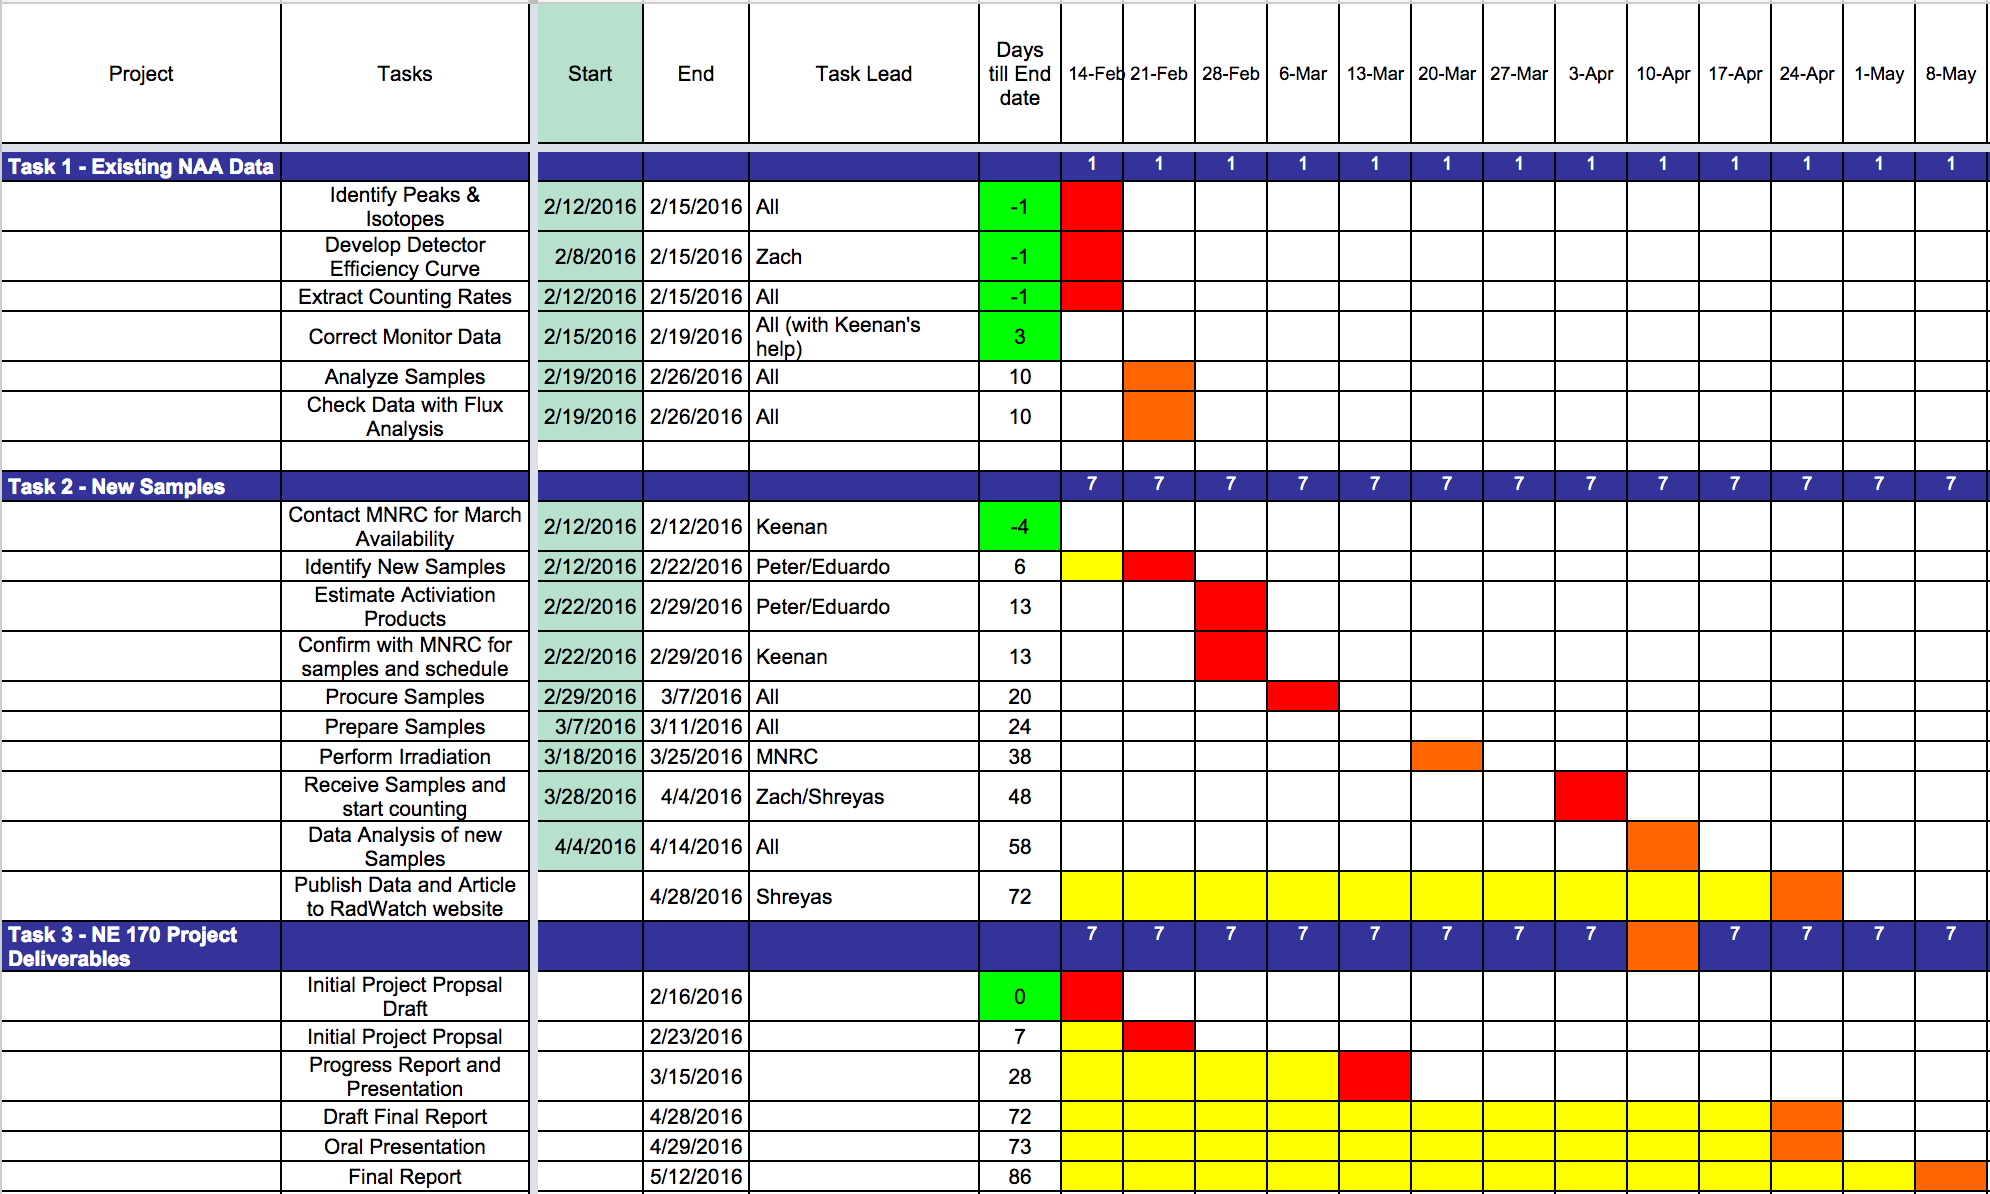
\includegraphics[scale=0.4]{GanttChart}
\caption{This figure shows a Gantt chart with the expected timeline to finish the various tasks for this project.}
\end{figure} 

\pagebreak

\section{Critical Equipment}
We will be using the following instruments/tools:


\begin{itemize}
\item High Purity Germanium (HPGe) Detector in 1110C
\item PeakEasy 4.81
\item MNRC reactor

Additional equipment will be added to this section as we move along with the project

\end{itemize}

\section{Irradiation Procedure}
\subsection{Long Run Procedure}

For the long run, we used samples of fish, seaweed, and seashells in order to diversify our sample data and findings.  Again, after receiving approval from MNRC to perform long run irradiation on our samples, we took the samples to MNRC.  The samples were placed in the NTD position, which has a lower flux, but allows for irradiation at a power level of 1 MW for many hours, as opposed to the PTS.  After waiting a few days for the samples to decay to safe levels, we received the samples in Etcheverry and counted them using the HPGe detector in the 1110C laboratory.
\section{Initial Research}
\subsection{Spectra Analysis}

\subsection{Short Run Procedure}
For the short run, we used four samples from the initial set of kelp samples.  After receiving clearance from MNRC to run these samples for a short-lived isotope test, we brought the samples to MNRC.  We put our sample vials inside rabbit tubes, which eventually went in the pneumatic transfer system (PTS).    The PTS is used for the short run, whereas the neutron transmutation doping position (NTD) is used for the long run.  See Figure *insert figure number based on report* for the locations of the PTS and NTD.  We ran the reactor at a power level of 20 kW, for a total of 100 seconds of irradiation.  Immediately after the samples decayed to a level safe to handle, MNRC ran counts on the samples up to an hour in length.  

*Insert Figure whatever here* (same picture as on Slide 16 currently in our presentation)



Figure 2 shows a sample spectra that we have already analyzed. Our initial analysis found the characteristic gamma rays of ${82}$Br and ${24}$Na. This shows that ${81}$Br and ${23}$Na were most likely present in our original sample, and using the neutron flux, neutron capture cross section, counts in peak, and detector efficiency, we can determine the initial composition of ${81}$Br and ${23}$Na in our sample.

\begin{figure}[h]
\centering
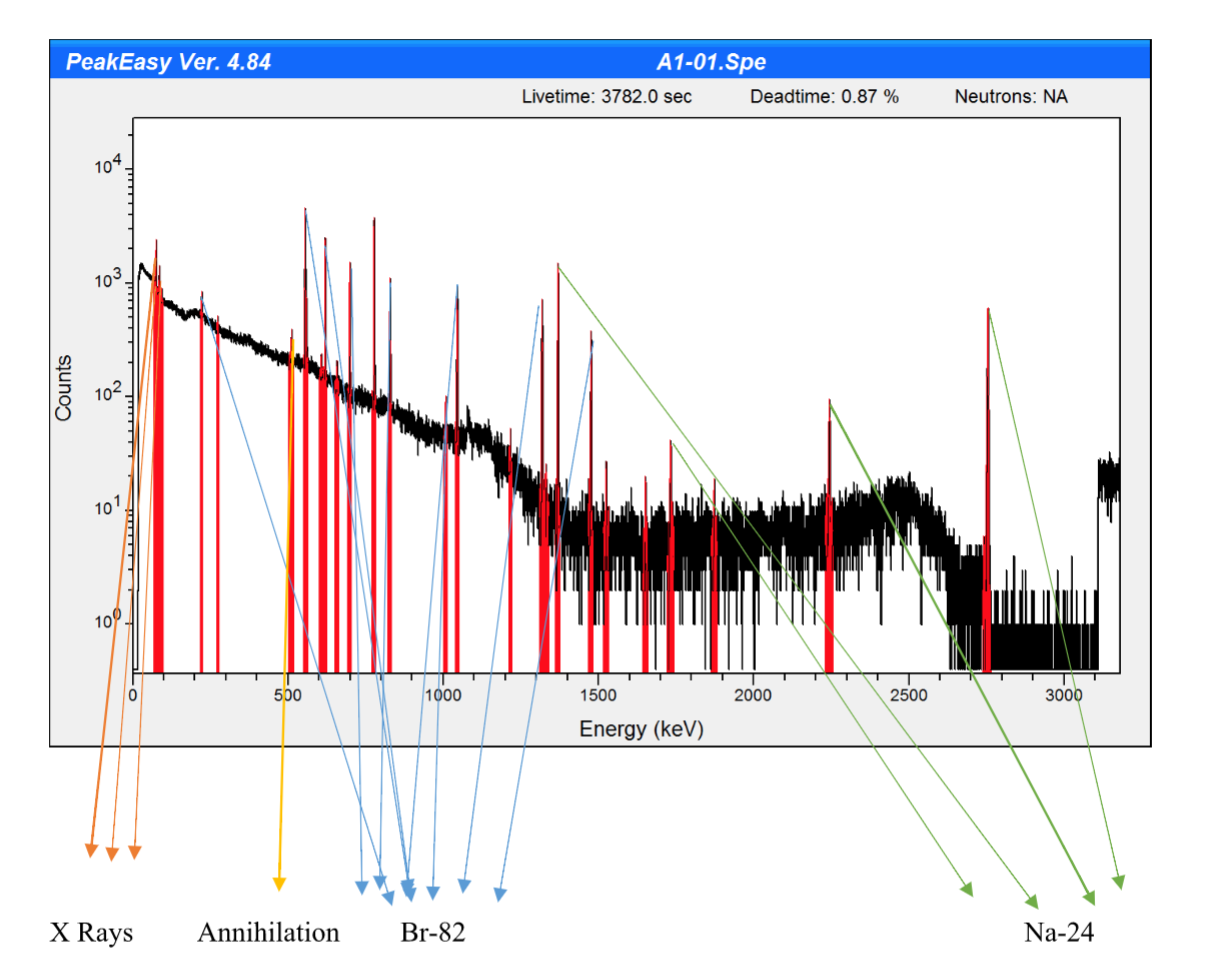
\includegraphics[scale=0.5]{ExampleSpectra}
\caption{This figure shows a NAA spectra for sample 1. $^{82}$Br and $^{24}$Na are very prominent in the spectra.}
\end{figure} 

\pagebreak


\subsection{Detector Efficiency Curve}

Figure 3 shows the detector effiency curve for the HPGe detector used in room 1110C. The sources used to generate the efficiency curve were $^{137}$Cs, $^{60}$Co, $^{152}$Eu, $^{22}$Na, and $^{228}$Th. We used a plethora of sources in order to cover a wide range of gamma ray energies and find the efficiency over the entire energy spectrum we will be measuring. Using this efficiency curve, we will be able to determine the inital elemental concentrations of our samples.


\begin{figure}[h]
\centering
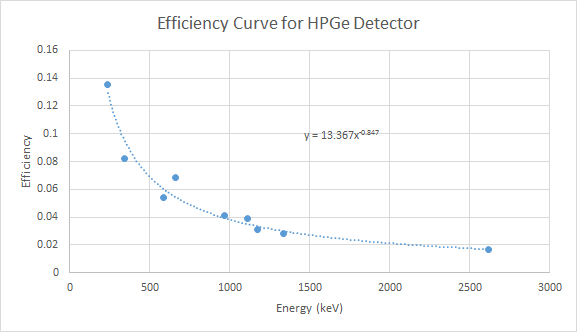
\includegraphics[scale=0.6]{Efficiency}
\caption{This figure shows the dectector efficiency curve for the HPGe detector in room 1110C.}
\end{figure} 

\pagebreak
 

\section{Data Analysis and Results}
\subsection{Concentration Calculation}

\begin{figure}[h]
\centering
\fbox{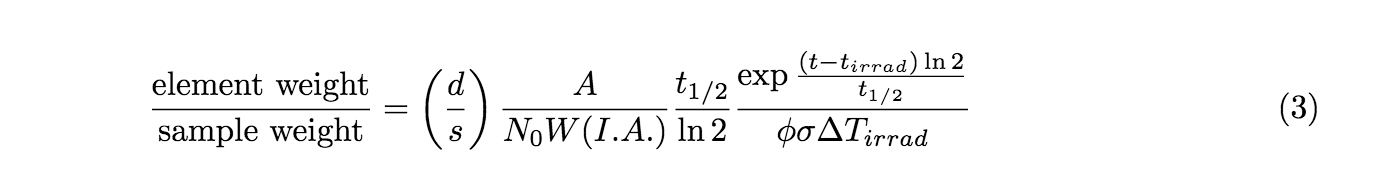
\includegraphics[scale=0.5]{Eq3}}
\caption{This figure shows the orthodox equation used to determine the relative abundance a given element in an unknown sample.}
\end{figure}

The orthodox way to determine relative elemental composition in an unknown sample is given by the equation in figure 4. However, by using standard pottery, we are able to determine the elemental composition of an unknown sample without detector efficiency, irradiation flux, and cross section. Standard pottery is clay pottery which contains a wide range of chemical elements. Using NAA, we can activate the pottery and use it as a chemical fingerprint for many different elements. Many minor components of the pottery are activated via NAA and these component compositions are known to high accuracy, making the standard pottery a valuable tool in determining the composition of an unknown sample. Figure 5 shows the elemental composition of the standard pottery used as part of this project.

\begin{figure}[h]
\centering
\fbox{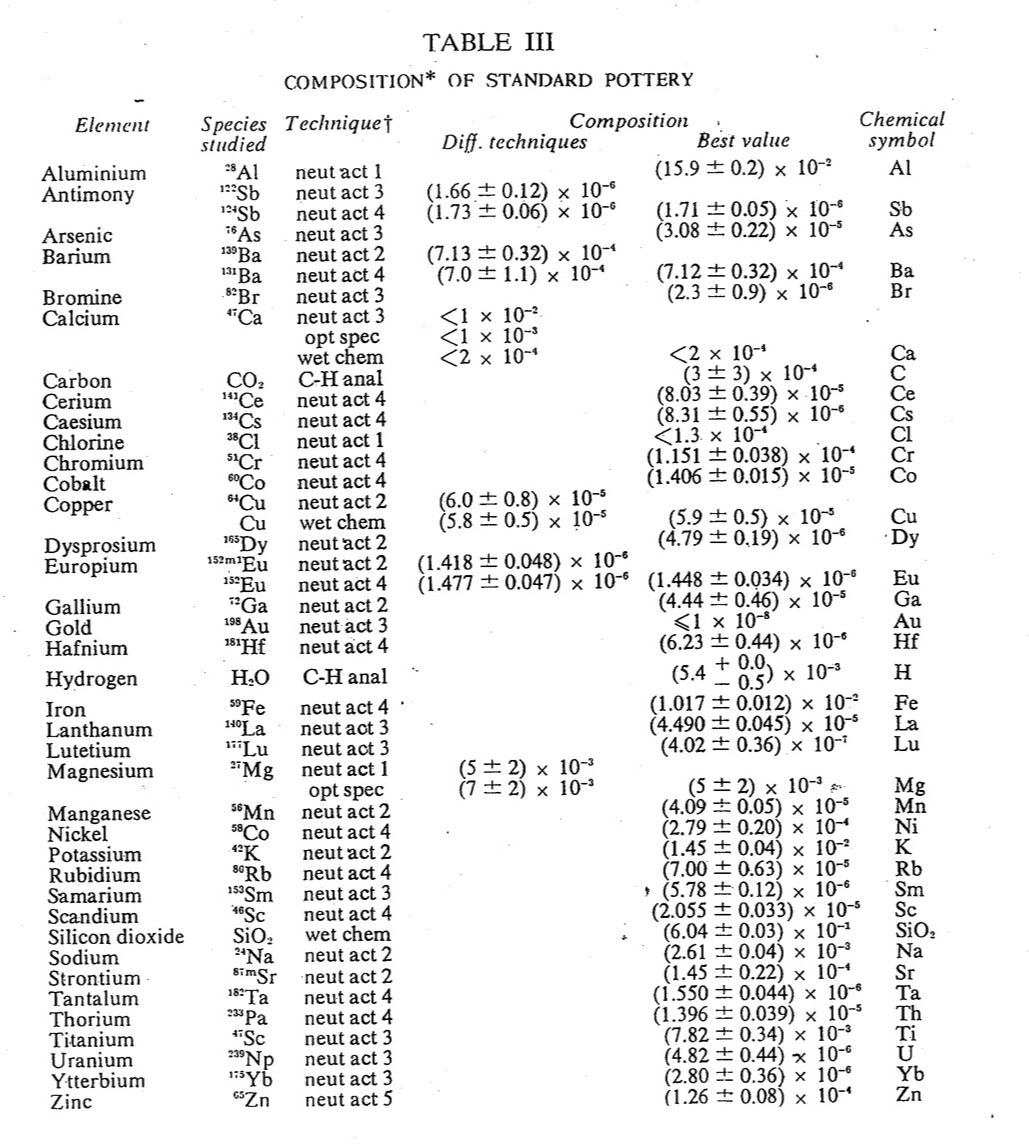
\includegraphics[scale=0.3]{stdpottery}}
\caption{This figure shows the orthodox equation used to determine the relative abundance a given element in an unknown sample.}
\end{figure}

The counts per second per gram, or $\frac{cps}{g}$ for a given sample is given by $$\frac{cps}{g} = \frac{N\Phi\sigma(1-e^{-\lambda t})\epsilon \beta_{ \gamma}}{m * LT}$$ where N is number of atoms, $\Phi$ is irradiation flux, $\sigma$ is cross section, $\epsilon$ is detector efficiency, $\beta_{\gamma}$ is branching ratio, LT is live time, and m is sample mass. We can write the activity A of a given sample as $$A=N\Phi\sigma(1-e^{-\lambda t})$$, allowing us to rewrite $\frac{cps}{g}$ of a given sample as $$\frac{cps}{g} = \frac{A\epsilon\beta_{\gamma}}{m*LT}$$ Using a simple ratio between level of sample activation and elemental concentration $\frac{A}{C}$, we can say that $$\frac{\frac{cps}{g}_{sample}|_{t=0}}{C_{sample}} = \frac{\frac{cps}{g}_{pottery}|_{t=0}}{C_{pottery}}$$ Using this ratio, we can calculate the elemental concentration in a given sample with the standard pottery. $$C_{sample} = \frac{\frac{cps}{g}_{sample}|_{t=0} C_{pottery}}{\frac{cps}{g}_{pottery}|_{t=0}}$$

The error associated ratio method for calculating sample concentration can be calculated using the error propagation formula $$\sigma_F^2 = \sum_{i=1}^N (\frac{dF}{dx_i})^2 \sigma_{x_i}^2$$. Expanding this out for the formula given above, we get that the error in concentration can be given by $$\sigma_{C_{sample}}^2 = (\frac{C_{pottery}}{\frac{cps}{g}_{pottery}|_{t=0}})^2\sigma_{\frac{cps}{g}_{sample}}^2 +  (\frac{\frac{cps}{g}_{sample} C_{pottery}}{(\frac{cps}{g}_{pottery})^2})^2|_{t=0}\sigma_{\frac{cps}{g}_{pottery}}^2 +  (\frac{\frac{cps}{g}_{sample}|_{t=0}}{\frac{cps}{g}_{pottery}|_{t=0}})^2\sigma_{C_{pottery}}^2$$

\begin{table}[h]
\centering
\caption{ This table shows the elemental compositions of the initial kelp NAA and error.}
\resizebox{\columnwidth}{!}{
\begin{tabular}{ | l | l | l | l | l | l | l |}
\hline
	Kelp ID & Sample Location & \% $^{42}$K & \% $^{24}$Na  & \% $^{82}$Br & \% $^{76}$As & \% $^{86}$Rb \\ \hline
	Sitka-1 & Sitka, AK & \  & \  & \  & \  & \  \\ \hline
	RES-1 & Tofino, BC & \  & \  & \  & \  & \  \\ \hline
	BML-1 & Van Damme State Park, CA & 3.81 $\pm$ 0.46  & 3.69 $\pm$ 0.07  & 0.064 $\pm$ 0.025  & 0.007 $\pm$ 0.0006  & \  \\ \hline
	UCSCTER-1 & Santa Cruz, CA & \  & \  & \  & \  & \  \\ \hline
	CAM-1a & Cambria, San Luis Obispo County, CA & \  & \  & \  & \  & \  \\ \hline
	REED-1c & Santa Barbara, CA & \  & \  & \  & \  & \  \\ \hline
	Oxy-1 & Rancho Palos Verdes, Los Angeles County, CA & 6.77 $\pm$ 0.61 & 3.22 $\pm$ 0.62 & 0.08 $\pm$ 0.03 & 0.008 $\pm$ 0.006 & \  \\ \hline
	LB-1 & Long Beach, Los Angeles County, CA & \  & \  & \  & \  & \  \\ \hline
	OI-1 & San Clemente, Orange County, CA & \  & \  & \  & \  & \  \\ \hline
	PTL-1 & Point Loma (San Diego), CA & 6.49 $\pm$0.73 & 3.10 $\pm$ 0.064 & 0.061 $\pm$ 0.024 & 0.0084 $\pm$ 0.0007 & 0.0047 $\pm$ 0.0006 \\ \hline
	UABC-1 & Baja California, Mexico & \  & \  & \  & \  & \  \\ \hline
	UCN-1 & Chile & \  & \  & \  & \  & \  \\ \hline
	LB-2B & Long Beach, Los Angeles County, CA & 5.43 $\pm$ 0.24 & 4.10 $\pm$ 0.07 & 0.14 $\pm$ 0.06 & 0.007 $\pm$ 0.0005 & 0.0018 $\pm$ 0.0002 \\ \hline
	NS6 & \  & \  & \  & \  & \  & \  \\ \hline
	NS1 & \  & \  & \  & \  & \  & \  \\ \hline
\end{tabular}

}
\end{table}


\subsection{Kelp Sample Long Run Results}

\subsection{Kelp Sample Short Run Results}

\subsection{Fish Long Run Results}

\subsection{Seaweed Long Run Results}

\subsection{Seashell Long Run Results}

\section{Conclusion}
\subsection{Isotope Identification}
Eduardo will be the primary author

\section{Future Work}
Shreyas will be the primary author


\section{Next Steps}
  
Once the isotopic composition of our test samples is known, we can research effects that the radioactive and chemically toxic isotopes can have on people’s health and the environment. This will hopefully give a better understanding of how harmful isotopes are transported through the oceans to different locations on the coast, and how we can combat the buildup of hazardous material along the coastline. This is in large part motivated by the Fukushima accident and the radiological release caused by that. Little was known prior to the accident about how radioactive isotopes are carried through the ocean, or how the concentration of these isotopes builds up in sea life. Because of this, the public was misinformed on the radiological impact of the Fukushima accident. This project is, in part, designed to address this misunderstanding. The NAA spectra results we obtain will be compared with the gamma-ray counting experiments performed by the RadWatch team earlier to verify accuracy. With the samples analyzed, and isotopic compositions noted, we can then find other samples of interest and compare the results. These results should give us some insight how the geography of the coast lines and the biology of the test samples chosen affect the isotope concentrations. We will also be able to see what effects human activity have on isotope concentrations, specifically how heavy industry in the Long Beach area contributes to the buildup of radioactive and toxic isotopes in the environment. The important findings from these experiments will be posted on the RadWatch website to assist with their research into radioisotope activity in the oceans. Hopefully, these findings will give some insight into what affects the concentrations of isotopes in ocean going samples, which will allow later teams to devise plans on how to best predict and combat buildup of hazardous materials along the coast. 

\section{Acknowledgements}

We would like to thank Keenan Thomas and Professor Kai Vetter for helping us determine the scope of this project, and for the assistance they give us during the course of completing this project. Furthurmore, we would like to thank Wesley Frey and the rest of the MNRC staff for assisting us with the irradiation. Finally, we would like to thank Max Fratoni for his guidance and assistance during the NE170 course and the completion of this project.


\end{document}




